% Model các cái này ra:
% Rating, efficiency, capacity, loa, cost, lifetime
% e the bay gio la sau khi tim duoc cai thiet bi dien roi ay, se thu duoc nhung gia tri nao? (kieu la tong kwh, cai continuous cao nhat (la khi nhieu appliances dung cung mot luc), va cai instantaneous dung ko))
First, we need to analyse the specifications of different batteries. There are many brands and types of battery chemistry commercially available. Therefore, before installing the batteries in our photovoltaic system, we need to consider our choices:
\begin{enumerate}
    \item Lead-acid batteries
\end{enumerate}
Lead-acid battery is the most popular and reliable chemistry used in a PV storage system, as it has been around since the 19th century. The stored chemical potential energy in the battery can be converted to electrical energy through the following reaction:

$$\mathrm{Pb}+\mathrm{PbO}_{2}+2 \mathrm{H}_{2} \mathrm{SO}_{4} \rightarrow 2 \mathrm{PbSO}_{4}+2 \mathrm{H}_{2} \mathrm{O}$$
$$
E^{0}=2.041 V
$$
, in which the voltage produced from the reaction is $2V$.\cite{wiki:lead_acid_battery}

There are many different lead-acid batteries available for solar arrays, and these batteries offer different solutions to our energy needs. After researching online for lead-acid batteries, here are our choices when modeling the 

\begin{enumerate}[resume]
    \item Lithium-ion batteries (primarily lithium cobalt oxide)
\end{enumerate}
Lithium-ion batteries, despite being more expensive than their lead-acid counterpart, are more efficient and allow more depth of discharge than their counterpart, thus being more cost-effective in the long run. Via separating the lithium ions from the electrons via an electrolyte, the electron therefore can be directed through a circuit in order to discharge the chemical potential energy inside.\cite{wiki:li_ion_battery} \\

\begin{enumerate}[resume]
    \item Lithium iron phosphate (LFP) batteries
\end{enumerate}
LFP battery is a type of lithium-ion battery that uses lithium iron phosphate instead of lithium cobalt oxide as cathode material. While the energy density and voltage of this type of battery is lower than that of traditional lithium-ion battery, it is generally safer, cheaper, has higher discharge rate and has more life cycle than that of lithium-ion does.\cite{wiki:lfp_battery}\\ 

With all of that in mind, we decided to choose 10 batteries, with 4 being lead-acid batteries, 4 being lithium-ion batteries and 2 being lithium iron phosphate batteries. This is because we need to test a variety of battery in order to find the most optimal choice between different batteries.
\newpage
\paperwidth=\pdfpageheight
\paperheight=\pdfpagewidth
\pdfpageheight=\paperheight
\pdfpagewidth=\paperwidth
\headwidth=\textheight
\begingroup 
\vsize=\textwidth
\hsize=\textheight
\begin{figure}[H]
    \centering
    \textbf{Table 4:} Specifications of multiple batteries
    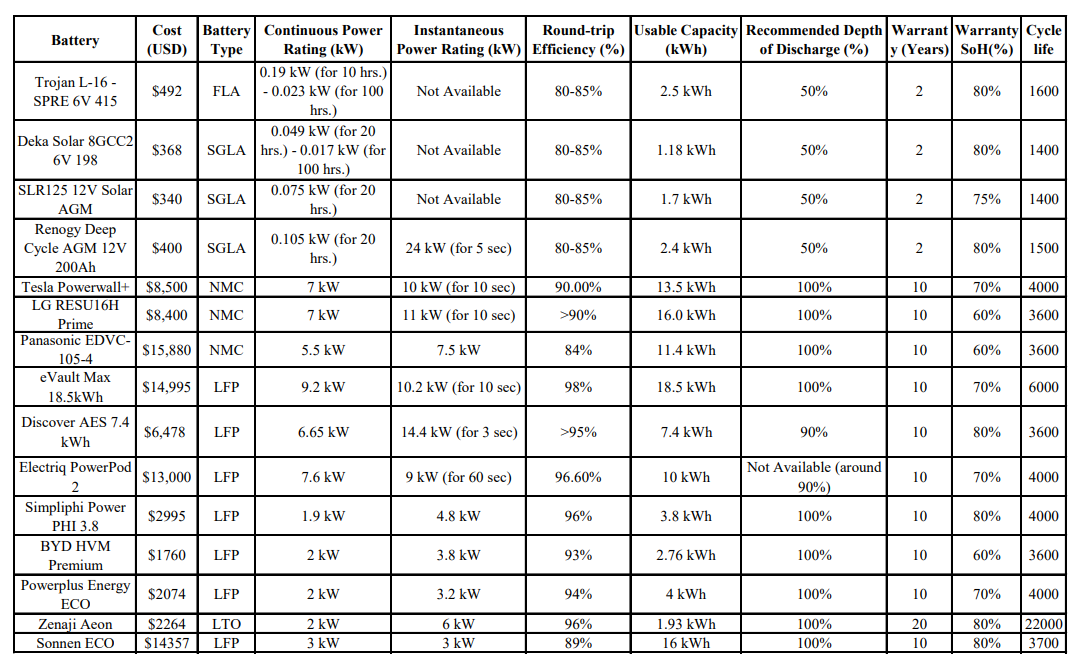
\includegraphics[scale=1.25]{src/aa.png}
\end{figure}

\endgroup
\newpage
\paperwidth=\pdfpageheight
\paperheight=\pdfpagewidth
\pdfpageheight=\paperheight
\pdfpagewidth=\paperwidth
\headwidth=\textwidth

\begin{comment}
\newgeometry{a3paper}
\paperwidth=\pdfpageheight
\paperheight=\pdfpagewidth
\pdfpageheight=\paperheight
\pdfpagewidth=\paperwidth
\headwidth=\textheight
\begingroup 
\vsize=\textwidth
\hsize=\textheight
% Table generated by Excel2LaTeX from sheet 'Sheet1'
\begin{table}[H]
  \centering
  \caption{Currently available battery models}
    \begin{tabular}{|p{6.865em}|p{3.32em}|l|p{7.725em}|p{7.635em}|l|p{6.225em}|l|l|l|l|}
    \toprule
    \textbf{Battery} & \textbf{Cost (USD)} & \multicolumn{1}{p{3.09em}|}{\textbf{Battery Type}} & \textbf{Continuous Power Rating (kW)} & \textbf{Instantaneous Power Rating (kW)} & \multicolumn{1}{p{5.865em}|}{\textbf{Round-trip Efficiency (\%)}} & \textbf{Usable Capacity (kWh)} & \multicolumn{1}{p{8.275em}|}{\textbf{Recommended Depth of Discharge (\%)}} & \multicolumn{1}{p{4.045em}|}{\textbf{Warranty (Years)}} & \multicolumn{1}{p{4.045em}|}{\textbf{Warranty SoH(\%)}} & \multicolumn{1}{p{4.045em}|}{\textbf{Cycle life}} \\
    \midrule
    Trojan L-16 -SPRE 6V 415 & \multicolumn{1}{l|}{\$492 } & \multicolumn{1}{p{3.09em}|}{FLA} & 0.19 kW (for 10 hrs.) - 0.023 kW (for 100 hrs.) & Not Available & \multicolumn{1}{p{5.865em}|}{80-85\%} & 2.5 kWh & 50\%  & 2     & 80\%  & 1600 \\
    \midrule
    Deka Solar 8GCC2 6V 198 & \multicolumn{1}{l|}{\$368 } & \multicolumn{1}{p{3.09em}|}{SGLA} & 0.049 kW (for 20 hrs.) - 0.017 kW (for 100 hrs.) & Not Available & \multicolumn{1}{p{5.865em}|}{80-85\%} & 1.18 kWh & 50\%  & 2     & 80\%  & 1400 \\
    \midrule
    SLR125 12V Solar AGM & \multicolumn{1}{l|}{\$340 } & \multicolumn{1}{p{3.09em}|}{SGLA} & 0.075 kW (for 20 hrs.) & Not Available & \multicolumn{1}{p{5.865em}|}{80-85\%} & 1.7 kWh & 50\%  & 2     & 75\%  & 1400 \\
    \midrule
    Renogy Deep Cycle AGM 12V 200Ah & \multicolumn{1}{l|}{\$400 } & \multicolumn{1}{p{3.09em}|}{SGLA} & 0.105 kW (for 20 hrs.) & 24 kW (for 5 sec) & \multicolumn{1}{p{5.865em}|}{80-85\%} & 2.4 kWh & 50\%  & 2     & 80\%  & 1500 \\
    \midrule
    Tesla Powerwall+ & \multicolumn{1}{l|}{\$8,500 } & \multicolumn{1}{p{3.09em}|}{NMC} & 7 kW  & 10 kW (for 10 sec) & 90.00\% & 13.5 kWh & 100\% & 10    & 70\%  & 4000 \\
    \midrule
    LG RESU16H Prime & \multicolumn{1}{l|}{\$8,400 } & \multicolumn{1}{p{3.09em}|}{NMC} & 7 kW  & 11 kW (for 10 sec) & \multicolumn{1}{p{5.865em}|}{>90\%} & 16.0 kWh & 100\% & 10    & 60\%  & 3600 \\
    \midrule
    Panasonic EDVC-105-4 & \multicolumn{1}{l|}{\$15,880 } & \multicolumn{1}{p{3.09em}|}{NMC} & 5.5 kW & 7.5 kW & 84\%  & 11.4 kWh & 100\% & 10    & 60\%  & 3600 \\
    \midrule
    eVault Max 18.5kWh & \multicolumn{1}{l|}{\$14,995 } & \multicolumn{1}{p{3.09em}|}{LFP} & 9.2 kW & 10.2 kW (for 10 sec) & 98\%  & 18.5 kWh & 100\% & 10    & 70\%  & 6000 \\
    \midrule
    Discover AES 7.4 kWh & \multicolumn{1}{l|}{\$6,478 } & LFP   & \multicolumn{1}{l|}{6.65 kW} & \multicolumn{1}{l|}{14.4 kW (for 3 sec)} & >95\% & \multicolumn{1}{l|}{7.4 kWh} & 90\%  & 10    & 80\%  & 3600 \\
    \midrule
    Electriq PowerPod 2 & \multicolumn{1}{l|}{\$13,000 } & \multicolumn{1}{p{3.09em}|}{LFP} & 7.6 kW & 9 kW (for 60 sec) & 96.60\% & 10 kWh & \multicolumn{1}{p{8.275em}|}{Not Available (around 90\%)} & 10    & 70\%  & 4000 \\
    \midrule
    Simpliphi Power PHI 3.8 & \$2995 &       & 1.9 kW & 4.8 kW & 96\%  & 3.8 kWh & 100\% & 10    & 80\%  & 4000 \\
    \midrule
    BYD HVM Premium & \$1760 &       & 2 kW  & 3.8 kW & 93\%  & 2.76 kWh & 100\% & 10    & 60\%  & 3600 \\
    \midrule
    Powerplus Energy ECO & \$2074 & \multicolumn{1}{p{3.09em}|}{Li-ion} & 2 kW  & 3.2 kW & 94\%  & 4 kWh & 100\% & 10    & 70\%  & 4000 \\
    \midrule
    Zenaji Aeon & \$2264 & \multicolumn{1}{p{3.09em}|}{LTO} & 2 kW  & 6 kW  & 96\%  & 1.93 kWh & 100\% & 20    & 80\%  & 22000 \\
    \midrule
    Sonnen ECO & \$14357 &       & 3 kW  & 3 kW  & 89\%  & 16 kWh & 100\% & 10    & 80\%  & 3700 \\
    \bottomrule
    \end{tabular}%
  \label{tab:addlabel}%
\end{table}%
\endgroup
\newpage
\paperwidth=\pdfpageheight
\paperheight=\pdfpagewidth
\pdfpageheight=\paperheight
\pdfpagewidth=\paperwidth
\headwidth=\textwidth
\restoregeometry
\end{comment}
However, it will be very difficult for people who have not worked with either batteries or electrical devices before to assess the following table in order to find the "best" battery. Our team determine that there should be a rating system that is easy to understand, convenient for end-users but also accurate during evaluation, making the process of choosing a suitable battery for solar energy storage easier. Here are several factors and formulas our team has taken into consideration and a model that assesses multiple battery storage systems:

\begin{enumerate}
    \item Power rating
\end{enumerate}
We have the following formula:
\[
P_a = \frac{P_c \times 59 + P_i}{60} * \text{average usage per hour}
\]
, which returns the average power rating in relation to the continuous power rating, the instantaneous power rating and the average power consumed per hour. As the period of time which the device reaches peak power usage is very short (only one minute per hour), the rest of the time the device consumes power at a constant rate. Therefore, we can calculate the mean power when using the formula (59 * continuous power rating + instantaneous power rating), after which it is divided the correct coefficient (60 minutes in an hour, 59 minutes of constant power usage and one minute of peak power consumption).

%Rating cho cost : cost / lifetime = cost / (number of cycles / 365) Do các loại pin có thời hạn sử dụng khác nhau, cùng với việc giá cả khác nhau, nên rất khó để đánh giá trực tiếp chỉ dựa trên giá cả. Một lối đi hợp lý theo chúng tôi là tính số tiền bạn bỏ ra trung bình mỗi năm khi mua hệ thống pin này. Khi đã cố định được đơn vị, ta có thể dễ dàng so sánh xem chúng ta nên bỏ ra bao nhiêu tiền một năm là hợp lý. Vì trung bình mỗi cycle diễn ra trong một ngày, nên thời gian sử dụng pin sẽ xấp xỉ số cycle chia cho 365 ngày trong một năm. Từ đó, ta có công thức để tính rating cho giá tiền.
\begin{enumerate}[resume]
    \item Cost rating
\end{enumerate}
The cost rating is calculated through the following formula:
\[
C_r = \frac{\text{Cost}}{\text{Lifetime}} = \frac{\text{Cost}}{(N_c / 365)}
\]
Because each battery has different lifetime and cost, therefore it is difficult to directly evaluate based on the original price. We believe that calculating the average cost per year spent on the system is a reasonable choice. After fixing the unit, we can easily compare how much money we should spend per year. Since on average a day consists a cycle, as such the amount of time using battery is on estimate the number of cycles divided by 365 days in a year. From that, we are able to derive a formula to calculate the cost rating.
%Do chúng ta chủ yếu sử dụng pin khi không có ánh nắng mặt trời (LoA), nên hệ thống pin của chúng ta cần có dung lượng dự trữ tổng phù hợp với lượng điện chúng ta dùng đến trong thời gian đó (usage * LoA). Lượng điện dự trữ tổng của hệ thống pin có thể được tính dễ dàng bằng cách nhân số pin cùng loại với dung lượng của một pin. Từ đó, để tính được tỉ số phù hợp của dung lượng , ta sẽ có công thức …

\begin{enumerate}[resume]
    \item Capacity rating
\end{enumerate}
The capacity rating is calculated as follow:
\[
R_cap = \frac{N_b \times C_a}{E_daily \times L_a} 
\]
As we use the batteries mainly when there is no sunlight, which invokes the length of autonomy (LoA), our battery system need to store enough electricity to use during the duration of the LoA ($E_daily \times L_a$). The amount of electricity stored in the system can be calculated by multiplying the number of batteries with the capacity of the battery. Therefore, in order to find the ratio between capacity, we have the following formula:
\begin{equation}
    \text{minimum } SoH = \frac{L_a \times E_daily}{N_b \times C_a \times DoD \times RTE}
    SoH \text{decreasing rate} = \frac{1 - \text{warranty} SoH}{365 \times \text{warranty length}}
\end{equation}

%\begin{enumerate}
%    \item Total rating
%\end{enumerate}
%After calculating all these 